\section{Grasp Net Benchmarks}   
    \label{secGraspNet}
 
\begin{figure}
\begin{center}
{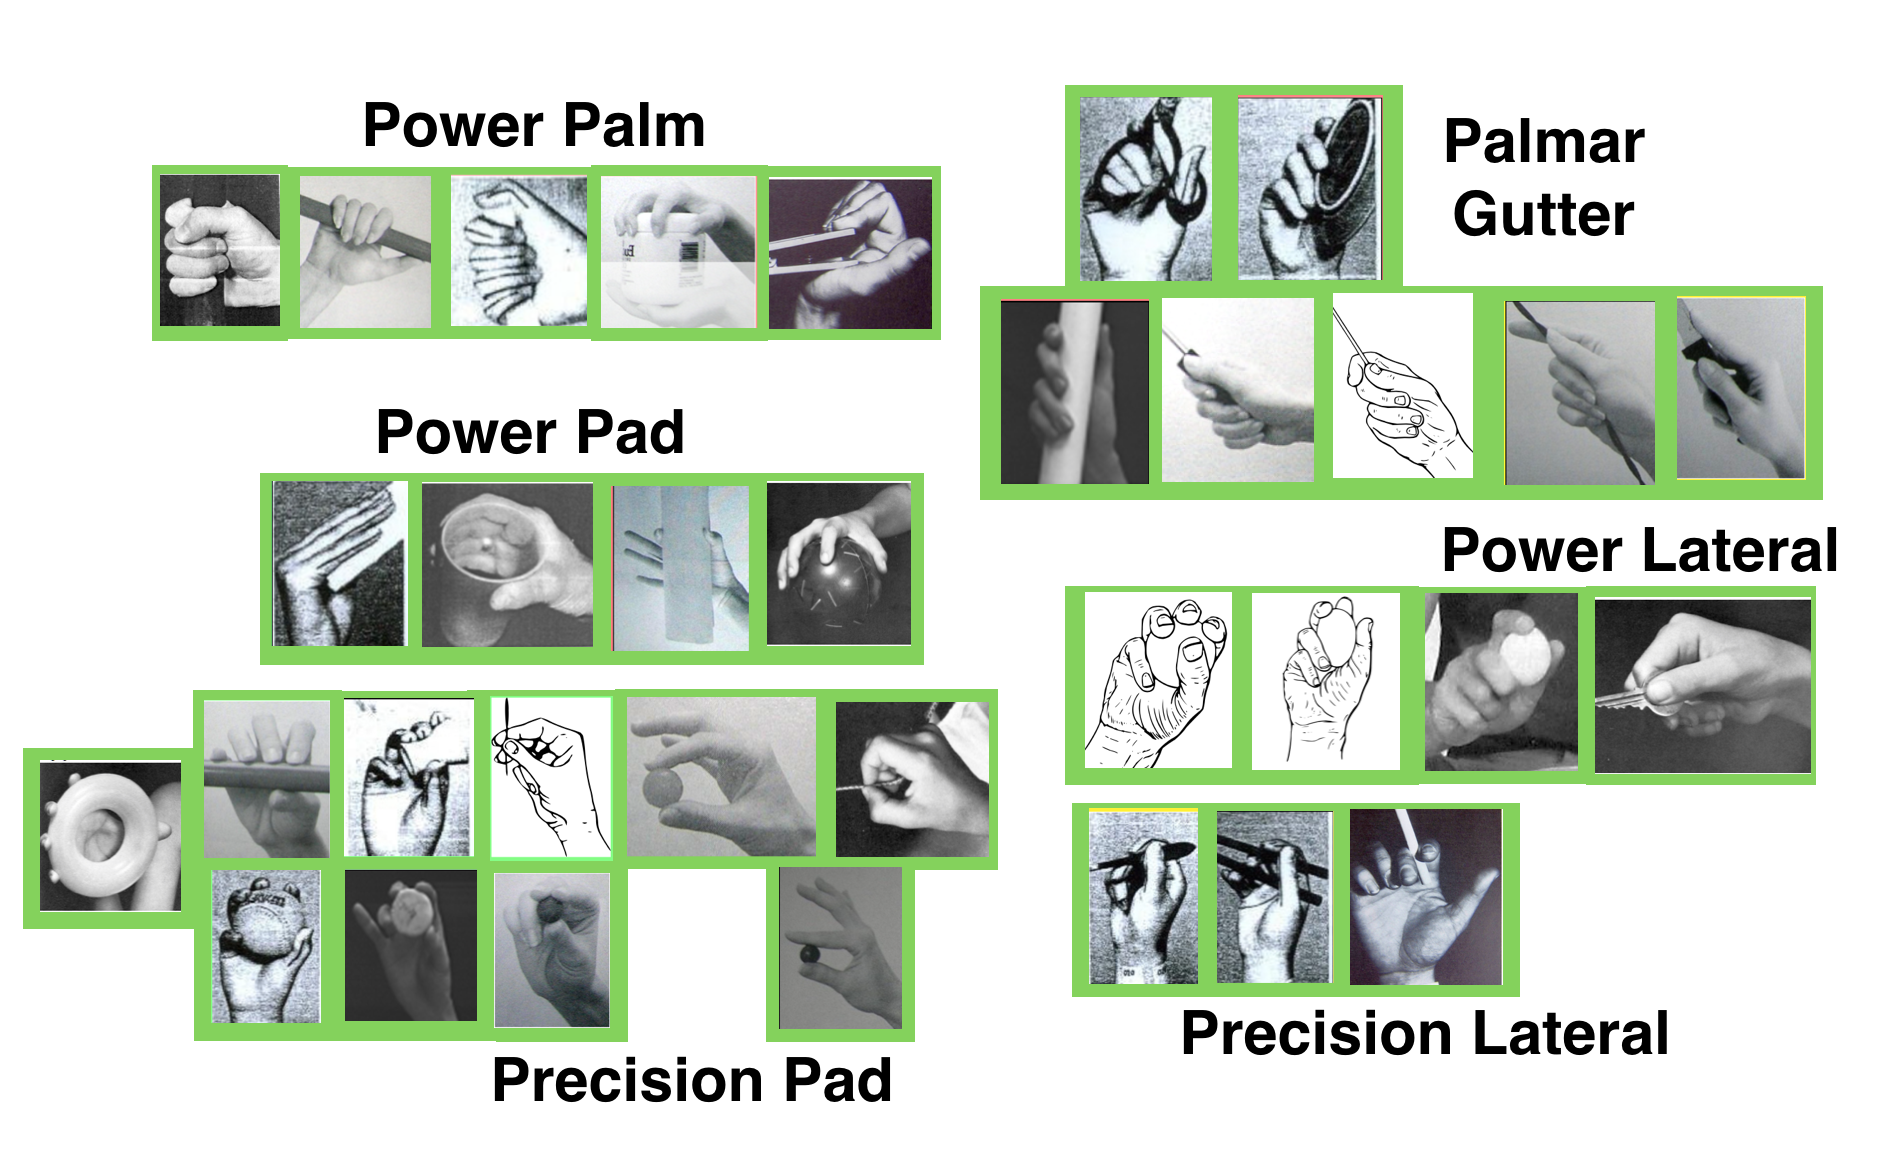
\includegraphics[height=2.2in]{./figs/sixGraspTypes.png}}
{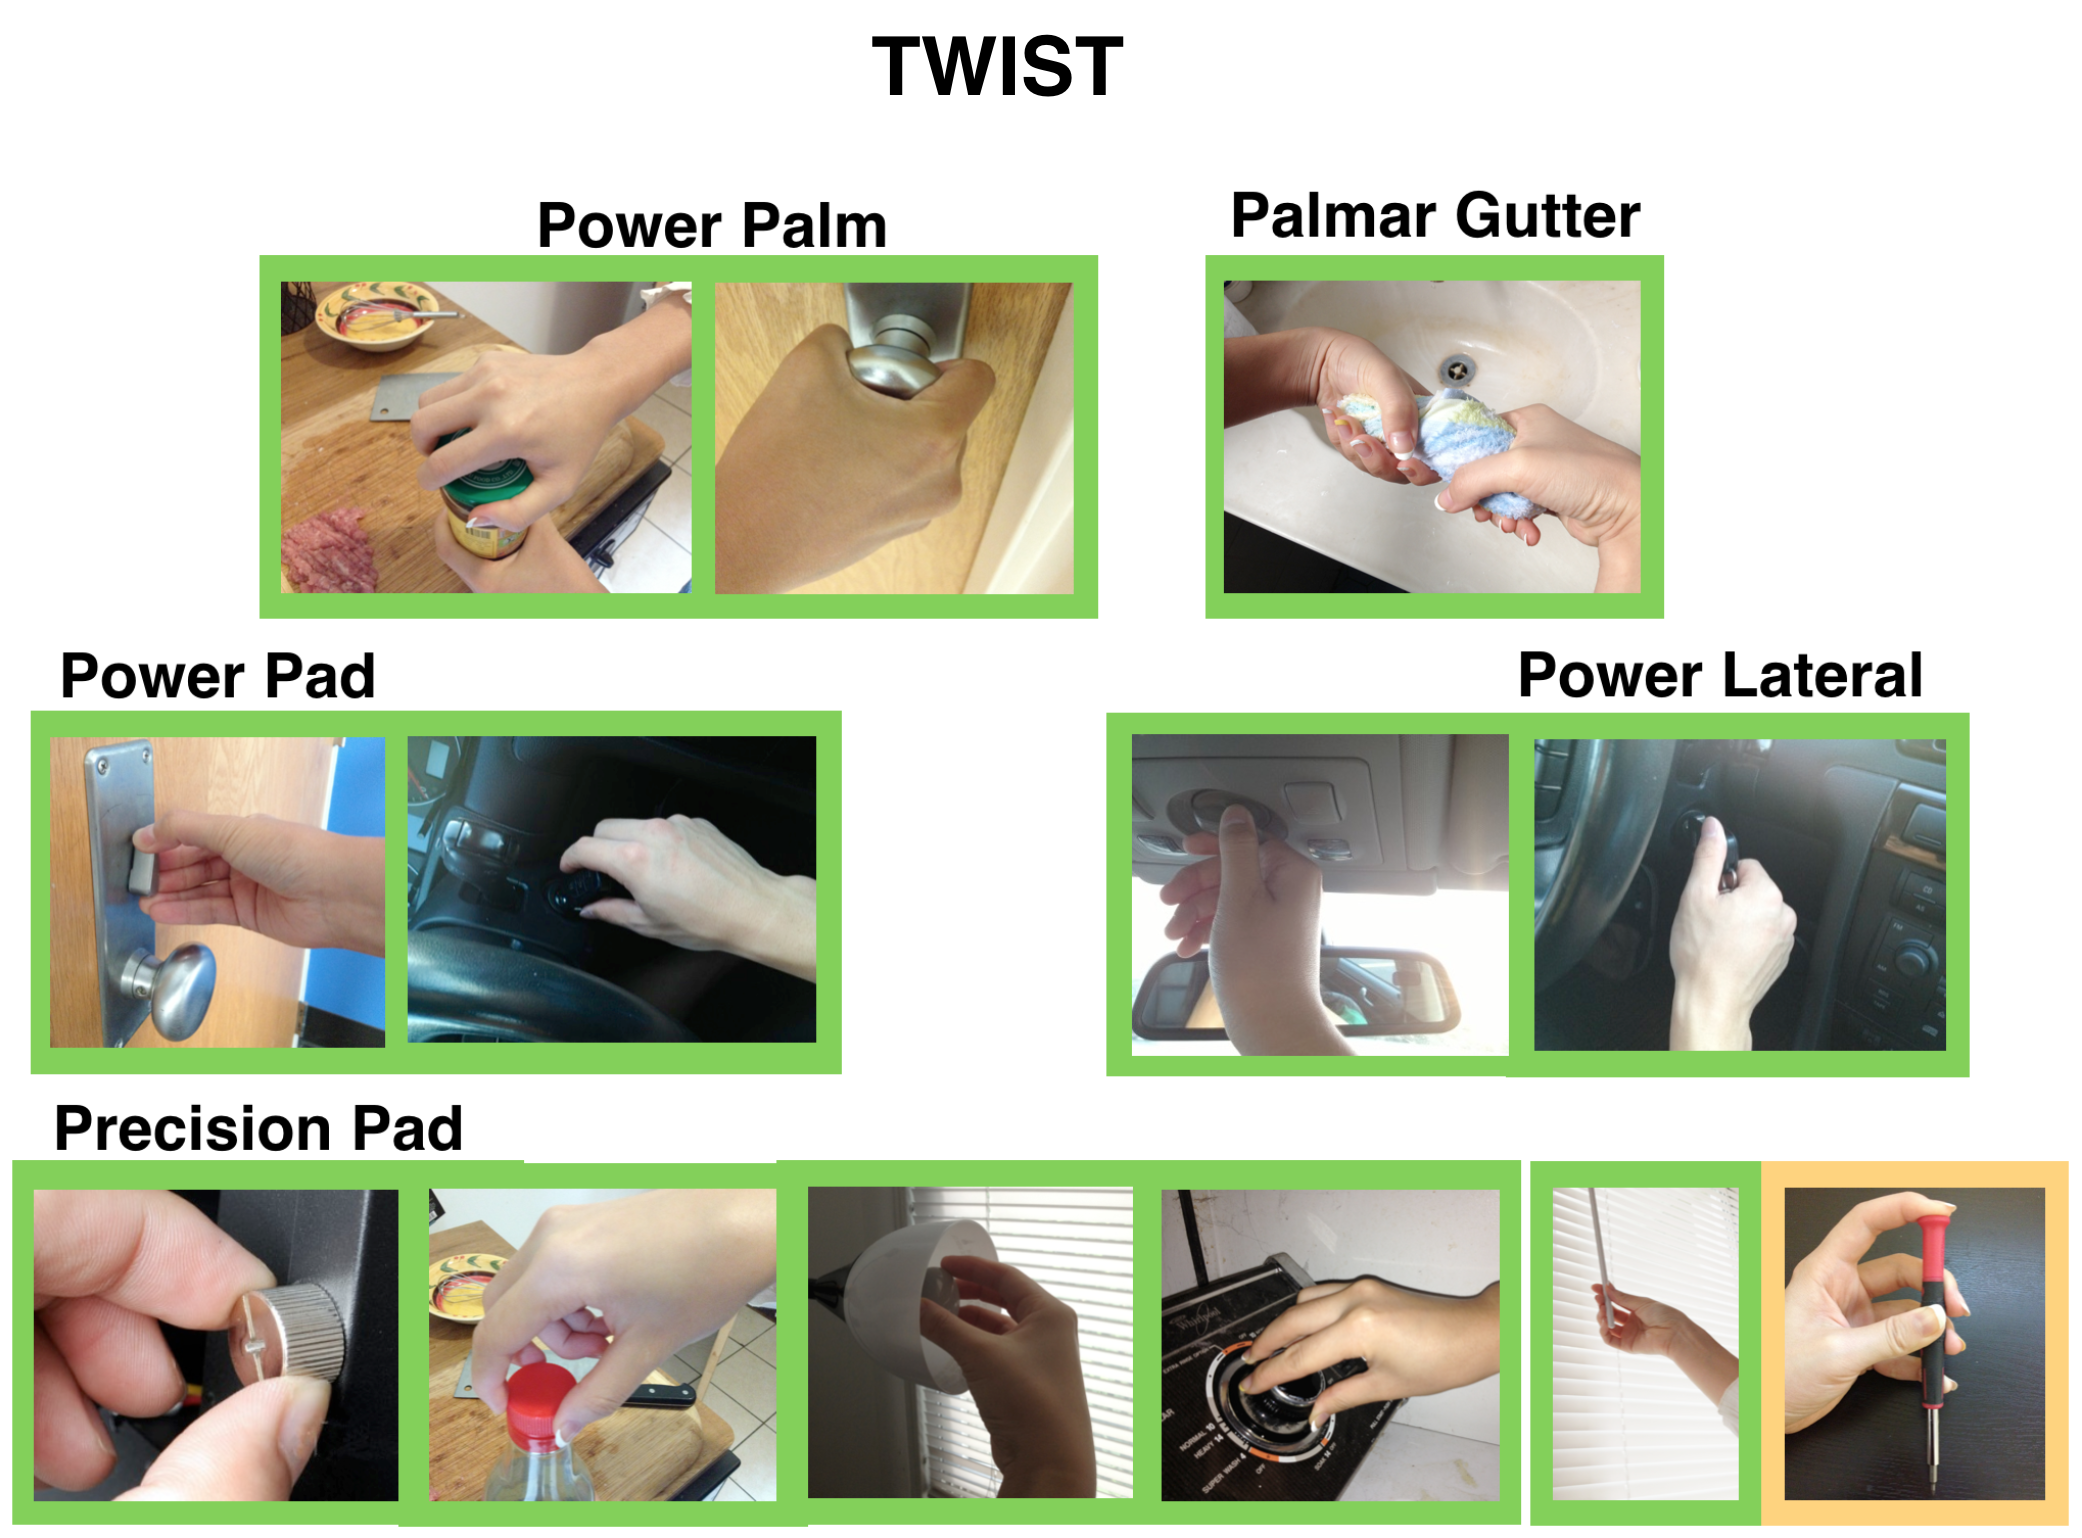
\includegraphics[height=1.8in]{./figs/twistGraspTypes.png}}
%{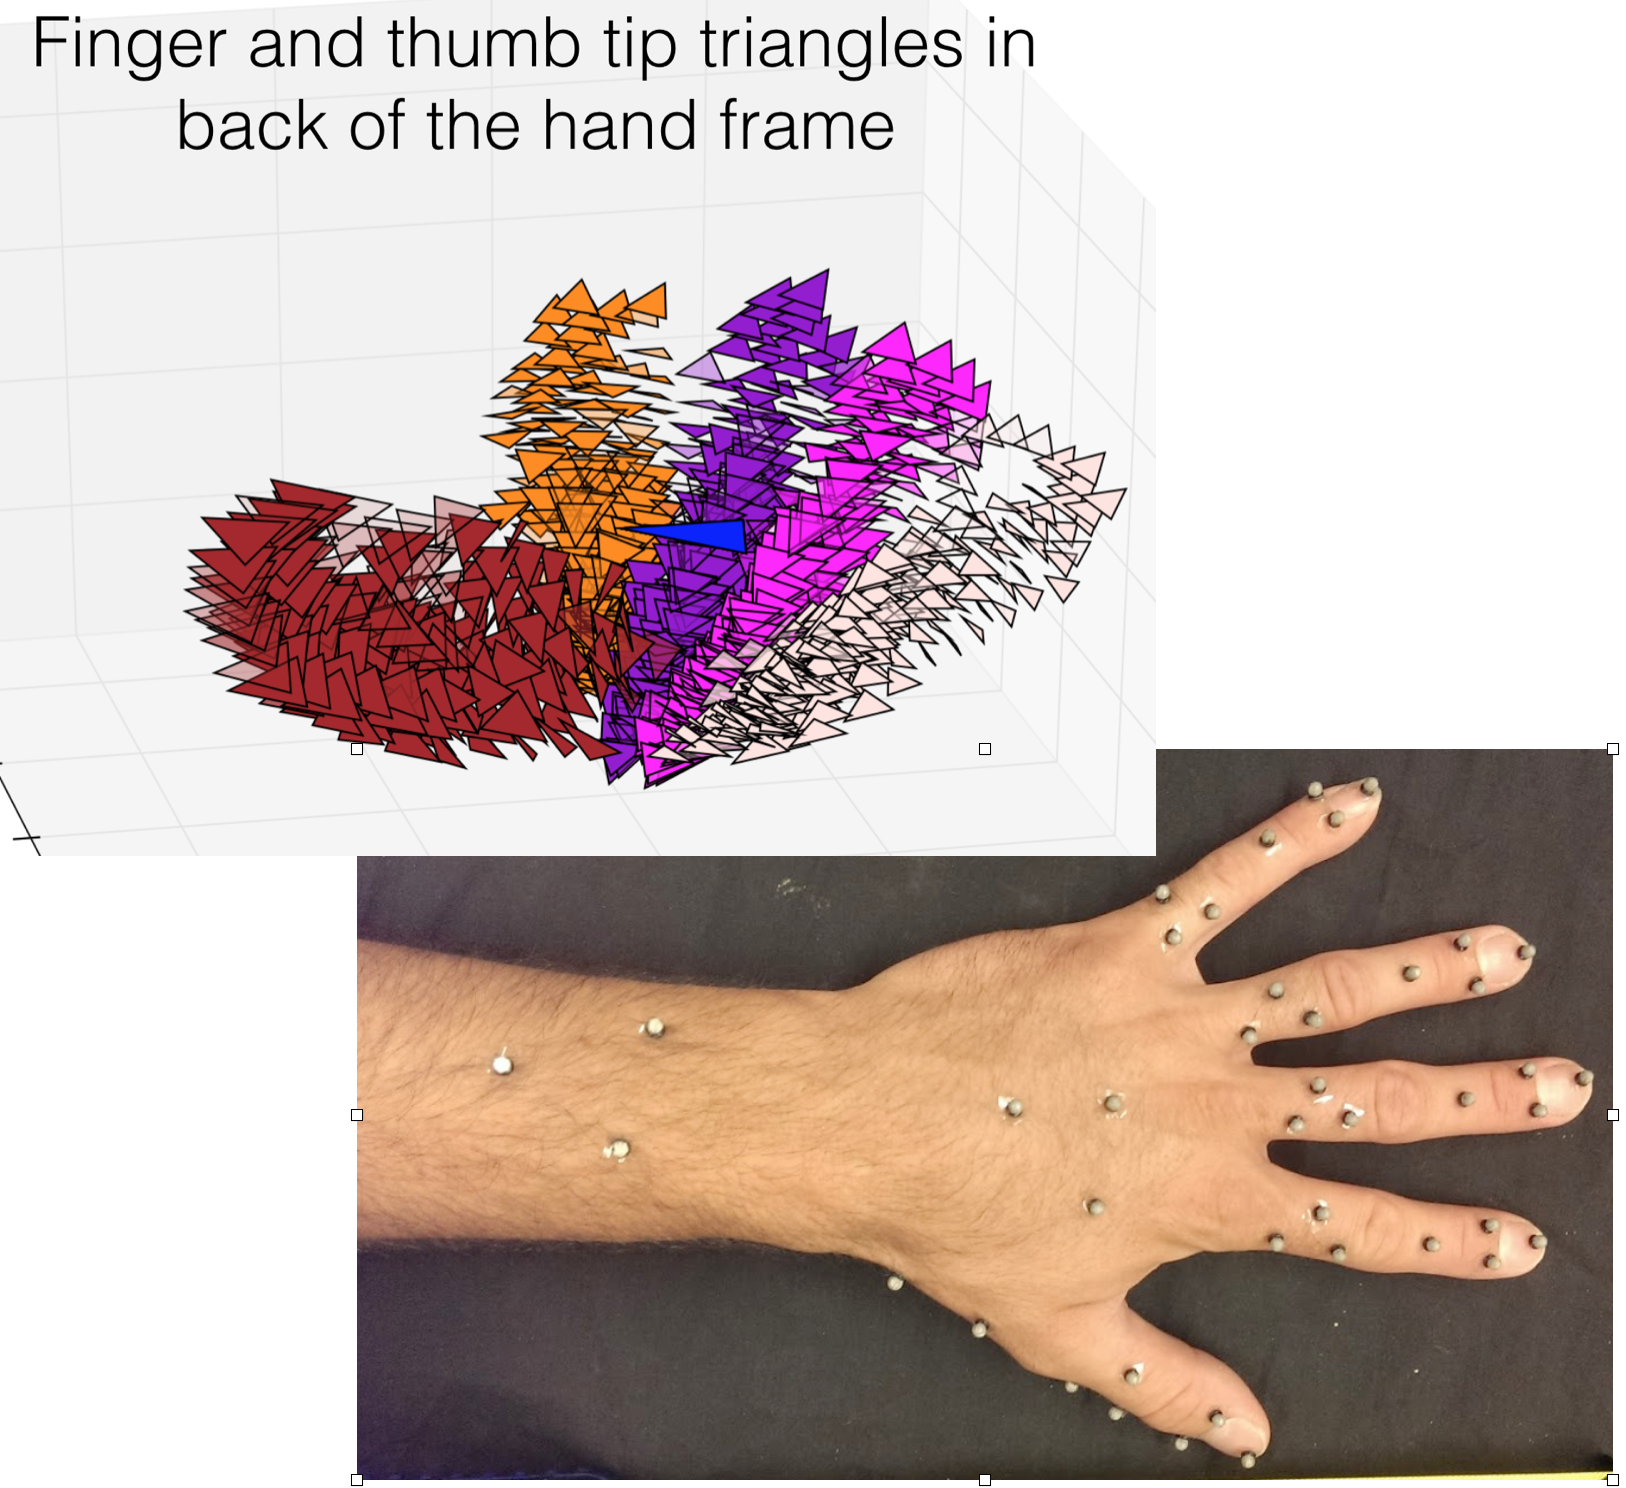
\includegraphics[height=1in]{./figs/mocap.png}}
\end{center}
\vspace*{-0.2in}
\caption[]{\small (Left) The 33 grasps of the Feix et al. taxonomy \cite{feixgrasp} can be grouped into six classes. (Right) Examples of 5 of these classes in use for the ``twist" action.}
\label{GraspNet}
\end{figure}

To tackle dexterous manipulation head-on, we must consider grasping and manipulation in its full complexity.   We take inspiration from human dexterity.   Full scale humanlike dexterous manipulation may appear enormously complex.   However,  we have observed a relatively small number of grasping tasks and manipulations that are used over and over, with common actions linked to one another, forming what we call Grasp Nets.   These Grasp Nets give us a way to proceed without oversimplifying.  We propose to create Grasp Net benchmarks to cover expanding portions of the dexterous manipulation space.   In tandem, we will develop evaluation procedures that test ability of a mechanism to accomplish Grasp Net tasks in the presence of uncertainty.   One project goal is to create and debug these tests to contribute them to the Roadmap to Progress Measurement Science in Robot Dexterity and Manipulation \cite{falco2014roadmap} where evaluation metrics for dexterous manipulation are needed.   

In this section, we provide some examples to illustrate the idea of a Grasp Net and some of the organizing principles we have observed through various human subject studies \cite{Liu2014, JiaDatabase, Chang:2009:RSSWorkshop, Chang:2014, liu2016annotating}.    These observations are as yet unpublished.

Consider first the grasp taxonomy recently developed by Feix and colleagues \cite{feixgrasp}, which pulls together the wealth of research on grasp classification over the last century.   There are 33 grasps in this taxonomy.  However, we find that they can be placed into six groups (Figure \ref{GraspNet}, Left).  Variations within a group depend mostly on object geometry, and occasionally function (scissors, knife, chopsticks).    Figure \ref{GraspNet}, Right shows examples of the ``Twist" action, uncovered in one of our studies \cite{liu2016annotating}.    Twist actions are found for five of the six categories.   Only the last, Precision Pad, requires intrinsic motions of the fingertips to achieve the twisting action.   In the remaining cases, most of the motion is performed by the wrist and/or arm.

We observe common transitions between the six grasping categories shown in Figure \ref{GraspNet}, such that a brief motion causes a robust transition from one grasp to another.   Figure \ref{DexterousExamples}, Right shows several examples, with the different colored arrows indicating some of the transition paths from one grasp to another.   Beyond  transitions between the six grasping categories, a Grasp Net must contain task related manipulations, such as the twist manipulations shown in Figure \ref{GraspNet} and manipulations to acquire and release an object.   One research challenge will be to map out benchmarks of GraspNet metrics of gradually increasing complexity, but such that each one provides full functionality for a set of tasks (e.g., the robot can get some family of objects into the hand, use them for their intended purpose, and put them back where it found them).

As preliminary work, we have collected detailed human motion data of a Grasp Net containing 21 grasps and more than 25 manipulations and have plans for several more such capture sessions.    Our marker set includes 39 markers on the hand and three on the forearm.    It is processed to a subject specific skeleton \cite{Chang:CoR06,Chang:AoR06,Chang:twoAxis08}.   Object models are available and object motions are tracked to allow estimates of likely contacts.  From these contacts, necessary, sufficient, and plausible families of contact forces can be estimated \cite{Li:graspDB07}.

